\documentclass{article}
\usepackage{tikz}
\usetikzlibrary{matrix,calc}
\begin{document}
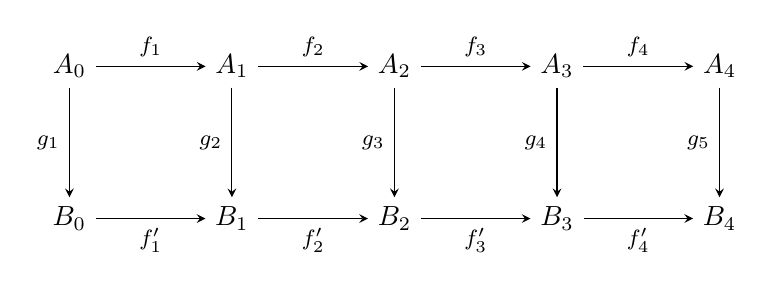
\begin{tikzpicture}[-stealth,
  label/.style = { font=\footnotesize }]
  \matrix (m)
    [
      matrix of math nodes,
      row sep    = 4em,
      column sep = 4em
    ]
    {
      A_0 & A_1 & A_2 & A_3 & A_4 \\
      B_0 & B_1 & B_2 & B_3 & B_4 \\
    };
  \foreach \i in {1,...,4} {
    \path
      let \n1 = { int(\i+1) } in
        (m-1-\i) edge node [above, label] {$f_\i$} (m-1-\n1)
        (m-2-\i) edge node [below, label] {$f^\prime_\i$} (m-2-\n1)
        (m-1-\i) edge node [left,  label] {$g_\i$} (m-2-\i);
  }
  \path (m-1-5) edge node [left, label] {$g_5$} (m-2-5);
\end{tikzpicture}
\end{document}